\documentclass{article}

\usepackage[a4paper, margin=20mm]{geometry}
\usepackage{cite}
\usepackage{amsmath,amssymb,amsfonts}
\usepackage[ruled, linesnumbered]{algorithm2e}
\usepackage{graphicx}
\usepackage{textcomp}
\usepackage{xcolor}
\usepackage{kotex}
\usepackage{multirow}
\usepackage{import}
\usepackage{fontspec}
\usepackage{hyperref}
\usepackage{float}

\setmainfont{함초롬바탕}
\setmainhangulfont{함초롬바탕}
\setsanshangulfont{함초롬바탕}
\setmonohangulfont{D2Coding}

\renewcommand{\refname}{참고문헌}

\begin{document}
\title{\textbf{실습 1. 초전형(Pyroelectric) 적외선 센서}\\
    \textbf{7조}
}
\author{
    권태환\\
    전자전기공학부\\
    \texttt{20234088}
    \and
    박상혁\\
    전자전기공학부\\
    \texttt{20234690}
    \and
    서유빈\\
    전자전기공학부\\
    \texttt{20223389}
    \and
    양가현\\
    전자전기공학부\\
    \texttt{20232549}
}
\date{2025.9.8.}
\maketitle

\section{실습 목적}
초전형 적외선 센서, LED, Op-Amp의 원리를 이해하고, 센서가 인체의 움직임을 감지하였을 때 발생하는 전압의 변화를 검출할 수 있는 초전형 센서 회로를 설계한다.

\section{실습 준비물}
\subsection{부품}
\begin{itemize}
    \item \textbf{적외선 센서 RE200B}: 1개
    \item \textbf{Op-Amp UA741CN}: 2개
    \item \textbf{LED}: 1개
    \item \textbf{커패시터 10nF, ceramic disk}: 1개
    \item \textbf{커패시터 10uF}: 2개
    \item \textbf{저항 100㏀, 1/2W, 5\%}: 1개
    \item \textbf{가변저항 10kΩ}: 2개
    \item \textbf{가변저항 1MΩ}: 2개
\end{itemize}

\subsection{사용장비}
\begin{itemize}
    \item \textbf{오실로스코프(Oscilloscope)}: 1대
    \item \textbf{브레드보드 (Bread board)}: 1개
    \item \textbf{파워서플라이 (Power supply)}: 1대
    \item \textbf{함수발생기 (Function generator)}: 1대
    \item \textbf{점퍼선}: 다수
\end{itemize}

\section{설계실습 계획서}
\subsection{초전형 적외선 센서(RE200B)와 증폭기 사이에 신호를 전달하는 High-Pass Filter(DC-block, 3-dB freq.=5 Hz)를 R과 C를 이용하여 설계하시오. (C 값은 10uF 고정)\label{sec1}}
\begin{figure}[H]
    \centering
    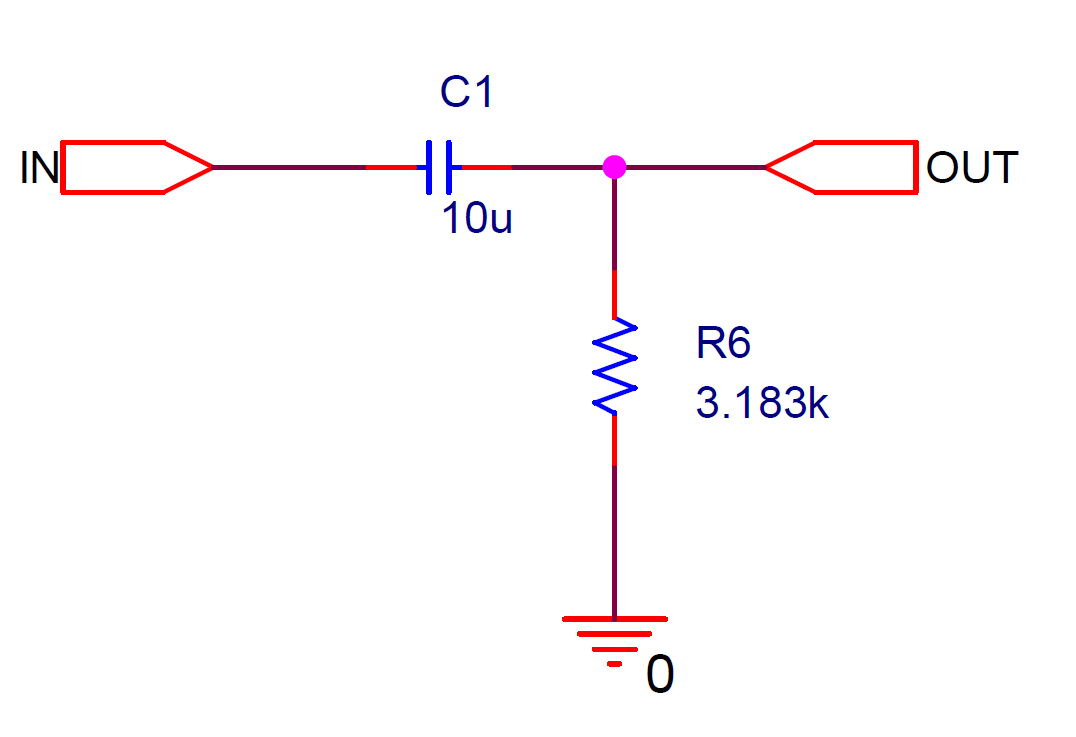
\includegraphics[width=0.5\linewidth]{figures/fig1.png}
    \caption{설계한 High-Pass Filter}
    \label{fig1}
\end{figure}
\cite{alexander2023fundamentals}에서 설명하는 RC High-Pass Filter 식을 사용하여 다음과 같이 계산할 수 있다.
주기와 주파수의 관계는 다음과 같다:
\[
    T = \frac{1}{f} = \frac{2\pi}{\omega}.
\]
차단 주파수 $\omega_c$에서의 관계식은
\[
    \omega_c = \frac{1}{RC}.
\]
여기서 커패시터는 $C = 10\,\mu\mathrm{F}$로 고정이므로,
\[
    R = \frac{1}{\omega_c C} = \frac{1}{2\pi f_c C}.
\]
주어진 $f_c = 5\,\mathrm{Hz}$를 대입하면,
\[
    R = \frac{1}{2\pi \times 5 \times 10 \times 10^{-6}}
    \approx 3.183\,\mathrm{k}\Omega
\]
이 된다. 해당 값을 바탕으로 회로를 그리면 Fig.~(\ref{fig1})이다.


\subsection{Op-amp 반전증폭기를 2-stage 로 연결하여 적외선 센서의 출력신호에 변화가 생길 경우 그 신호를 증폭시키는 회로를 설계하시오. (단, Gain 이 10000 V/V 가 되도록 설계하시오.)\label{sec2}}
반전 증폭기의 Gain은 \cite{alexander2023fundamentals}, \cite{ele}와 같이 구할 수 있다.
\begin{align}
    V_{out} = -\frac{R_f}{R_1}\cdot V_{in}
\end{align}
주어진 저항을 바탕으로 $R_2 = R_3 = 10k\Omega, R_4 = R_5 = 1M\Omega$ 으로 저항을 두고 Gain을 구하면 다음과 같다.
\begin{itemize}
    \item 첫번째 증폭 단에서 $-\frac{R_f}{R_1} = -\frac{R_4}{R_2} = -100$
    \item 두번째 증폭 단에서 $-\frac{R_f}{R_1} = -\frac{R_5}{R_3} = -100$
    \item 총 증폭 값 : $-100\times-100 = 10000~(V/V)$
\end{itemize}
해당 값을 적용한 증폭회로는 Fig.~(\ref{fig2})이다.

\begin{figure}[H]
    \centering
    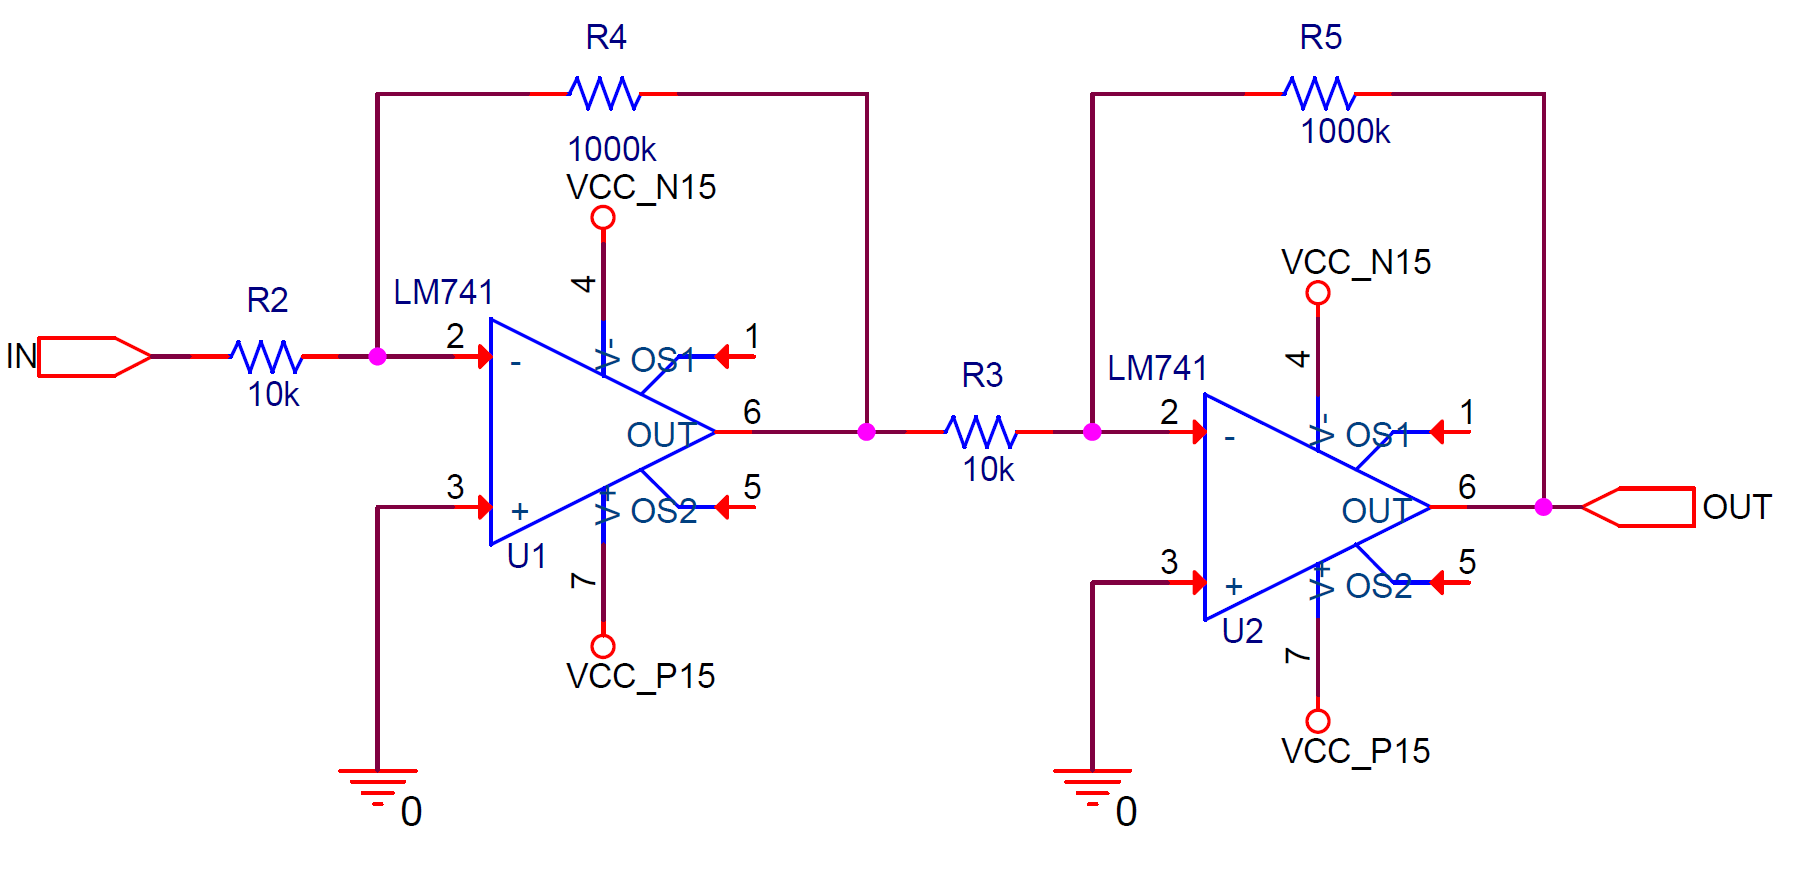
\includegraphics[width=0.7\linewidth]{figures/fig2.png}
    \caption{설계한 증폭 회로}
    \label{fig2}
\end{figure}

\subsection{\ref{sec2}의 Op-amp의 출력신호를 이용하여 센서의 움직임 검출 신호를 LED 점등으로 확인할 수 있는 회로를 추가하시오.}
\ref{sec1}, \ref{sec2} 에서 계산한 값을 바탕으로 회로도를 그리면 Fig.~(\ref{fig3})이다.

\begin{figure}[H]
    \centering
    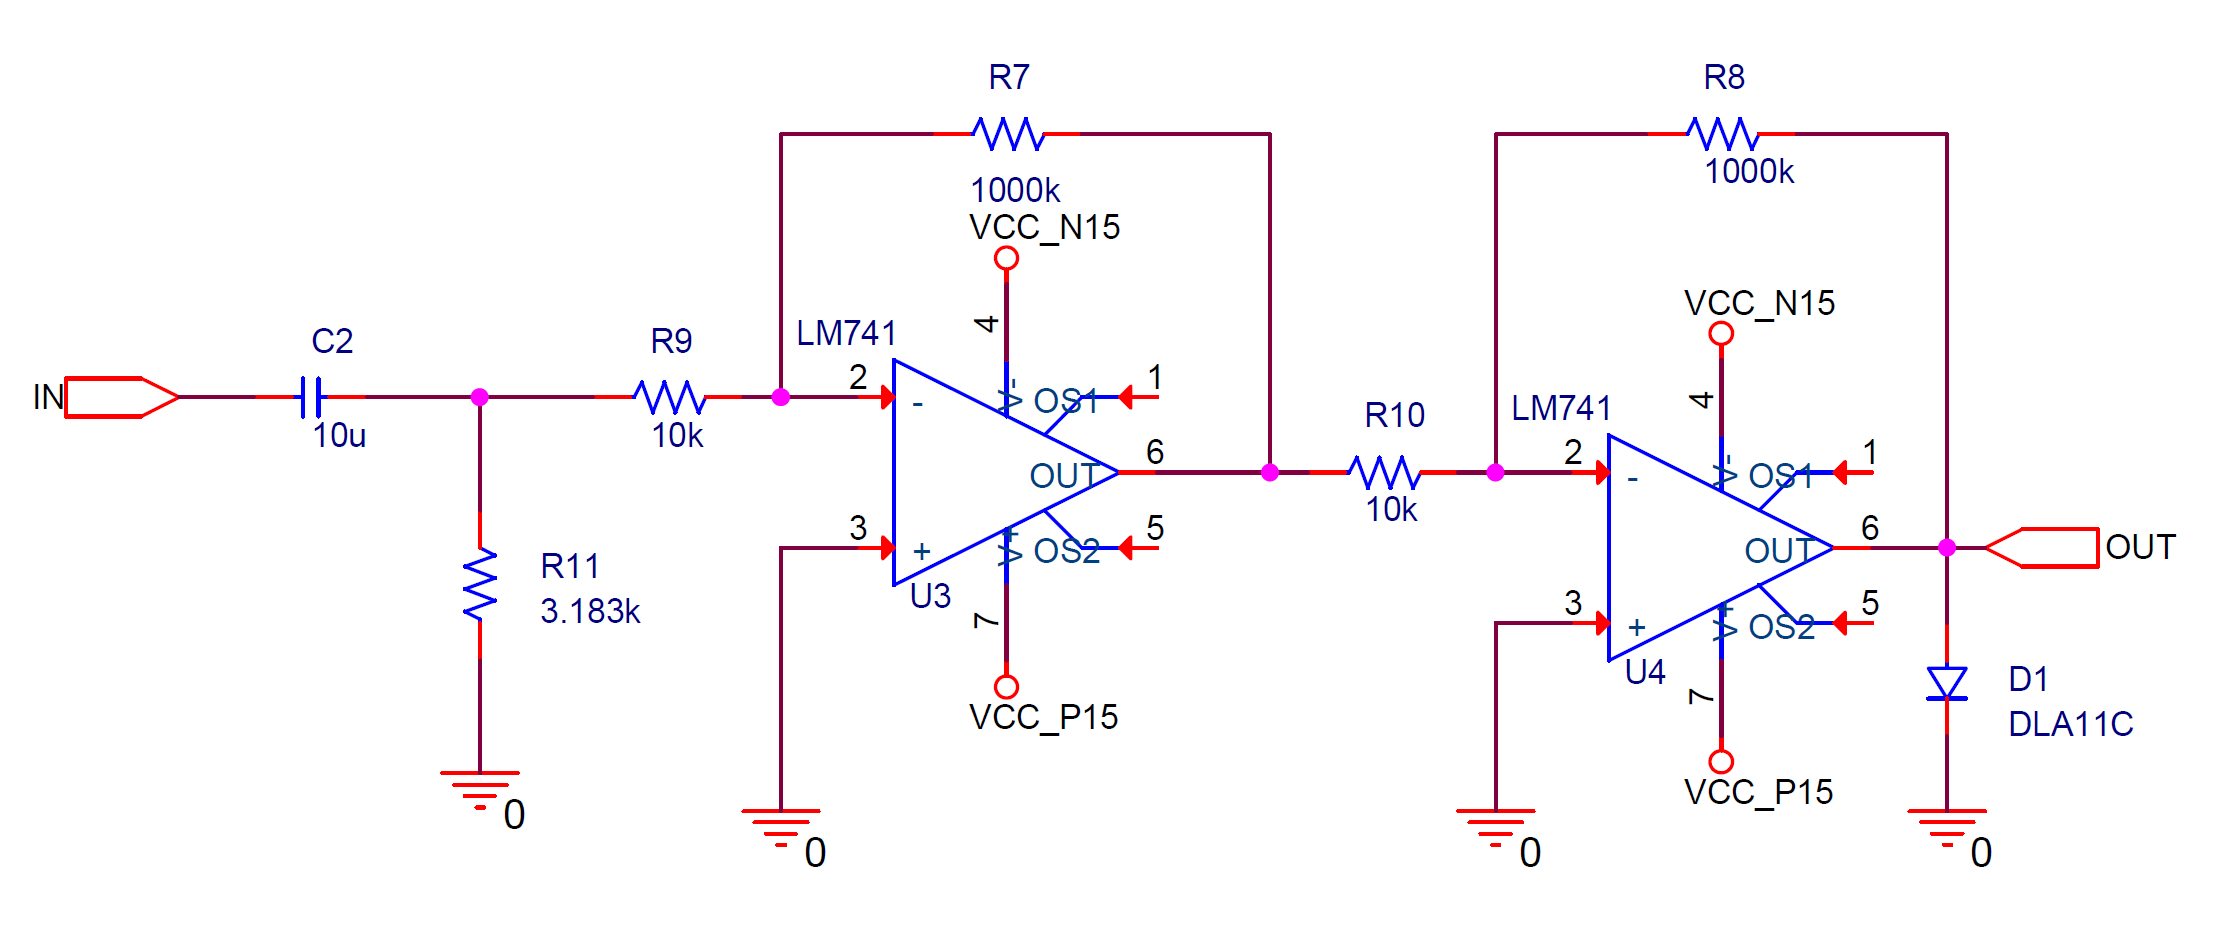
\includegraphics[width=0.7\linewidth]{figures/fig3.png}
    \caption{설계한 다이오드를 추가한 증폭 회로}
    \label{fig3}
\end{figure}


\bibliographystyle{plain}
\bibliography{refs}
\end{document}
